\documentclass[11pt, a4paper]{article}
\usepackage[turkish]{babel}
\usepackage{graphicx}
%\usepackage{natbib}
\usepackage{tcolorbox}
\graphicspath{ {./images/} }
%Tarih Ekleme
\usepackage{datetime}
\renewcommand{\dateseparator}{.}
\renewcommand{\figurename}{Şekil}
\renewcommand{\refname}{Kaynakça}


\title{El Biometrisinden Kişi Tanıma Projesi Tanıtımı}
\author{Ayşenur Şimşek\\ {aysesimsek920@gmail.com}}

\begin{document}
	
	\begin{figure}
		\centering
		
\includegraphics{ksbu.png}
	\end{figure}
	
	\maketitle
	
	\begin{center}
		Kütahya Sağlık Bilimleri Üniversitesi, Mühendislik ve Doğa Bilimleri Fakültesi, Bilgisayar Mühendisliği Bölümü, Kütahya, Türkiye \newline \newline
	\end{center}
	
	\pagenumbering{gobble}
	
\begin{enumerate}
    \item {\Large\textcolor{black}{Giriş}}
	\\Bu proje, insan elinden kişi tespiti yapmayı hedefleyen bir uygulama geliştirmeyi amaçlamaktadır. Günümüzde, güvenlik sistemlerinde ve benzeri uygulamalarda kişi tespiti ve tanıma önemli bir yer tutmaktadır.Kişisel kimlik doğrulamada güvenilirlik, havaalanı gözetiminden elektronik bankacılığa kadar birçok uygulama alanındaki sıkı güvenlik gereksinimlerinin anahtarıdır. İnsanların birçok fizyolojik özelliği, yani biyometri, tipik olarak zaman içinde değişmez, elde edilmesi kolaydır ve her birey için benzersizdir.\cite{kumar2006personal} Özellikle, insan elinin karakteristik özelliklerinin kullanılmasıyla kişi tanıma sistemleri daha güvenilir hale gelmektedir.
	
	Projenin belirlenmesindeki temel amaç, insan elinin görüntülerini kullanarak kişileri tanımlamak ve tespit etmek için bir yöntem geliştirmektir.\cite{shu1998automated} Bu yöntem, elin anatomik yapısını analiz ederek kişiye özgü özellikleri belirleyecek ve bu sayede kişileri doğru bir şekilde tanımlayabilecektir.
	
	Bu proje kapsamında, derin öğrenme ve görüntü işleme tekniklerinden faydalanılarak el görüntülerinin analiz edilmesi ve kişi tespiti için bir modelin oluşturulması planlanmaktadır. Bu model, elin genel şekli, parmak uzunlukları, parmakların arasındaki mesafe gibi özellikleri kullanarak kişileri tespit etme yeteneğine sahip olacaktır.\\
	
	\item {\Large\textcolor{black}{Literatür araştırması}} \newline
	Biyometrik modeller, bireylerin davranışsal veya fiziksel özellikleri ile otomatik tanımlama yapmamızı sağlar. Biyometrik yaklaşımlar içinde avuç içi, diğer modellere göre yeni bir biyometrik özelliktir. Avuç içi diğer biyometriklere göre bazı avantajları vardır:
	\begin{itemize}
		\item[$\bullet$] Düşük çözünürlüklü görüntüleme de kullanılabilir
		\item[$\bullet$] Düşük maliyetli kameralar görüntüyü elde etmek için yeterlidir
		\item[$\bullet$] Avuç içinin taklit edilmesi zordur
		\item[$\bullet$] Avuç içi özellikleri karakteristik ve kalıcıdır
	\end{itemize}
	Bu nedenlerden dolayı avuç içi tanıma sistemleri son zamanlarda araştırmacıların ilgisini çekmektedir.  El geometrisi üzerine yapılmış çalışmalardan başta avuç içi tanıma için de çeşitli yayınlarda çizgiye dayalı, dokuya dayalı  ve görünüşe dayalı yöntemlere dayanan birçok yaklaşım mevcuttur.  
	\begin{enumerate}
		\item BİYOMETRİK SİSTEMLER \\
		El geometrisi, kişi tanımada kişilerin el şekillerini kullanan bir biyometrik özelliktir. Bir biyometrik sistem de, el geometrisine dayanarak ana hat oluşturulur ve gerçekleştirilir. İşlem önceliği (siyah-beyaz içindeki renk görüntüsünü değiştirdiği gibi, ayrıt sezimi ve dış hatları çıkarma) ve ölçüm algoritmaları el görüntüsüne uygulanır. El geometrisi tanıma sisteminde üç temel birim vardır. 
		\item[$\bullet$] Bölütleme
		\item[$\bullet$] Özellik çıkarımı
		\item[$\bullet$] Tanıma \\
		Bölütleme: Bölütleme birimi, el ve parmakların dış hatlarını arka plandan çıkarır. İlk olarak giriş için renkli bir imge alınır. Sonra da sistem matlab’ın ―rgb2gray‖ fonksiyonu ile renkli görüntüyü gri seviyeye çevirir.\cite{ergen2011biyometrik}
		\begin{figure}[!h]
			\centering
			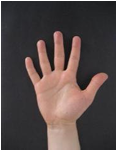
\includegraphics{el.png}
			\caption{El görüntüsü}
			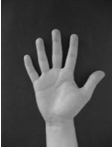
\includegraphics{griel.png}
			\caption{Gri el görüntüsü}
		\end{figure}
		\\Gri seviye imgesi eşikleme ile ikili sisteme dönüştürülür. Eşikleme gri seviyedeki bir imgeyi ikili sisteme çevirir. Belirlenen özel bir eşik değeriyle, eşik değerin altında veya yukarısındaki pikseller iki seviyede tanımlanır. Eşik değerinden büyük değerler 1(beyaz), küçük değerler ise 0(siyah) olarak ikili imgeye çıkış olarak verilir.\\
		\begin{figure}[h]
			\centering
			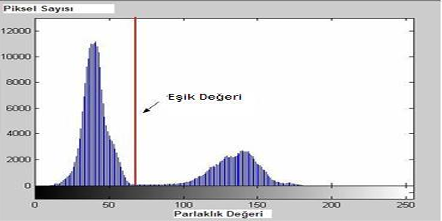
\includegraphics{histogram.png}
			\caption{Histogram ve eşik değeri}
		\end{figure}
		Özellik Çıkarımı: Özellik çıkarmanın amacı, el görüntüsünün özelliklerini elde etmektir. Özellik çıkarma birimi, parmakların uzunluklarını, genişliklerini, farklı uzunluktaki parmakları ve bir özellik vektörü olarak avuç içini bulur.  Bu özellikleri almak için, önerilen algoritma dış hat piksellerini ve onların konumunu kullanır.\\
		
		Tanıma: Son olarak tanıma birimi, veri tabanıyla özellik çıkarma vektöründen el de edilen giriş imgesini karşılaştırır. Böylece tanılama veya doğrulama için sonuçlar verilir.   Sistem, çıkarılan özellikleri kaydeder, tanıma işlemi için veri tabanıyla özellik vektörü eşleştirilir. Bir kişinin kimliğinin tanınması iki temel tipte sınıflandırılabilir: doğrulama ve teşhis. \cite{kong2002palmprint} Doğrulama, kimlik iddia eden kişiyi doğrular ya da reddeder. Doğrulama sisteminde, bireysel talepler, önceden sistemde kayıtlı olan kullanıcılar içindir. Sistem, veritabanında kayıtlı olan kişi ile o kişi olduğunu iddia eden kişiyi özellik vektörüyle(elde edilen veri) eşleştirerek onaylar veya reddeder. Böylece, doğrulama sistemi bire bir eşleştirme işlemi yapar.
		
	\end{enumerate}
	
	
	
	
	
	\item {\Large\textcolor{black}{Metodoloji}}
	
	Avuç İçi Görüntülerinin Toplanması: İlk adım olarak, veri setimizi yani görüntüleri farklı kişilerden kendimiz toplayarak bir klasörde tutacağız. Bu görüntüler, farklı açılardan ve farklı ışık koşullarında çekilecektir.
	
	Görüntü İşleme Tekniklerinin Uygulanması: Toplanan avuç içi görüntülerine, görüntü işleme teknikleri uygulanacaktır. Bu teknikler, görüntülerin düzeltilmesi, kenarların belirlenmesi ve özelliklerin çıkarılması gibi işlemleri içerecektir.
	
	Özellik Çıkarımı: Görüntüler üzerinde belirlenen özellikler, avuç içi geometrisinin karakteristik özelliklerini temsil edecek şekilde çıkarılacaktır. Bu özellikler, parmak uzunlukları, parmak aralıkları, avuç içi yapısı gibi parametreler olacaktır.
	
	Model Oluşturma: Elde edilen özellikler kullanılarak bir tanıma modeli oluşturulacaktır. Bu model, derin öğrenme veya makine öğrenmesi algoritmalarıyla eğitilecek ve farklı kişilerin avuç içi görüntülerini tanıyabilecektir.
	
	Doğrulama ve Değerlendirme: Oluşturulan model, farklı kişilere ait avuç içi görüntülerini tanıma yeteneğini değerlendirmek için doğrulama veri seti üzerinde test edilecektir. Modelin doğruluk oranı ve performansı değerlendirilecektir.
	
    \item {\Large\textcolor{black}{Veritabanı ve Veriler}} \newline %Sonuçlar-Tartışma
	
	
    \item {\Large\textcolor{black}{Beklenen Sonuçlar}}  \\ %Sonuç
	Güvenilir kimlik doğrulama günümüz dünyasında çok önemlidir. Avuç içi tarama teknolojisi diğer biyometrik sistemlere göre birçok avantaja sahiptir. Avuç içi, kolay ve maliyeti düşük teknolojiler ile gerçeklenme imkânı olduğundan uygulama açısından kolaylıklar içerir. Basit bir kullanıcı sistem etkileşimi sağladığı için sıfır veya çok küçük hatalı kayıt oranı elde edilebilir. Ayrıca avuç içi tarama teknolojisi yüksek kullanıcı kabulüne sahip.  Son olarak avuç içi tanıma sistemi, daha hızlı ve daha küçük avuç içi görüntüsü elde eden cihazla geliştirilebilir.\cite{kumar2006personal} Bu gelişimden sonra avuç içi tanıma sistemi sanayide kullanılıp ticari bir ürün haline gelebilir.
\end{enumerate}	
	  
	%Kaynakçayı yazdırmak
%\bibliographystyle{plain}
\bibliographystyle{ieeetr}
\bibliography{references.bib} 
%\printbibliography %Prints bibliography
\end{document}